\section{Umsetzung}
\label{sec:Umsetzung}
Im Anschluss an Kapitel \ref{sec:Grundlagen}, in dem die theoretischen Grundlagen erläutert wurden, beschreibt dieses Kapitel, wie die Grundlagen umgesetzt werden. Zuerst wird die Funktionsweise des Elastic Stacks erklärt. Dabei werden seine Komponenten schrittweise vorgestellt. Zum Abschluss des Kapitels wird auf die Implementierung des Apriori Algorithmus eingegangen.
%Nachdem wir in Kapitel \ref{sec:Grundlagen} die theoretischen Grundlagen für unser Vorhaben erläutert haben, wollen wir in diesem Kapitel beschreiben, wie die Grundlagen umgesetzt wurden.

\subsection{Grundlagen zum Elastic Stack}
\label{sub:Grundlagen zum Elastic Stack}
Um die Fragen aus der Problemstellung zu beantworten, wurde der Elastic Stack (ELK) benutzt. Der ELK besteht aus den Software Produkten Elasticsearch, Logstash und Kibana der Firma Elastic N.V. Zusätzlich wurde noch Filebeat von der gleichen Firma benutzt. Die Funktionen der einzelnen Produkte werden in den nachfolgenden Unterkapiteln weiter erläutert. Die folgende Abbildung stellt den Workflow des Systems dar:

\begin{figure}[htb]
\begin{center}
	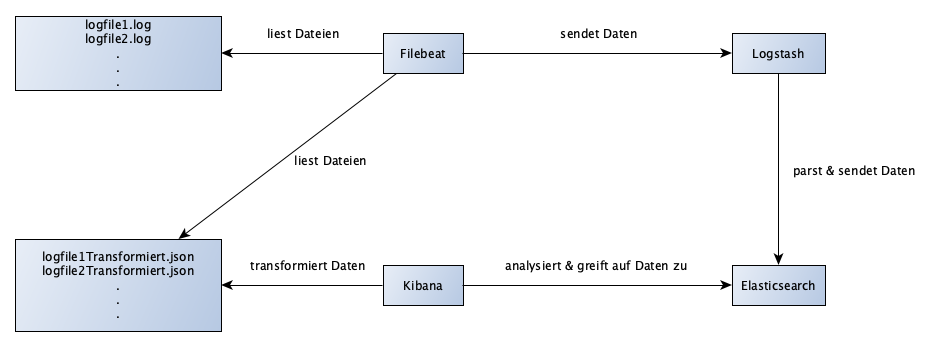
\includegraphics[width=440pt]{bilder/workflow.png}
\end{center}
\caption{ELK Workflow}
\label{fig:elk_workflow}
\end{figure}


\subsubsection{Filebeat}
\label{ssub:Filebeat}
Mit Filebeat können Dateien zeilenweise gelesen werden. In der Konfigurationsdatei von Filebeat gibt man an wo und nach welchen Dateiendungen gesucht werden soll. In unserem Fall waren es .log und .json Dateien. Außerdem kann man ein multiline pattern angeben, falls ein Eintrag mehrzeilig sein sollte. Die eingelesenen Dokumente sendet Filebeat an Logstash weiter. Dabei merkt sich Filebeat, welche Dateien schon gelesen wurden und wie weit diese gelesen wurden. Das bedeutet ebenfalls, wenn eine komplett neue Datei oder eine neue Zeile in einer alten Datei auftaucht, merkt Filebeat das, liest es und sendet die Daten wieder an Logstash \citep{ShuSha17}.
\subsubsection{Logstash}
\label{sub:Logstash}
Die Aufgabe von Logstash ist Daten von Filebeat zu empfangen und zu verarbeiten. Die empfangenen Daten befinden sich in einem rohen Zustand und werden mit Hilfe von mehreren Filter-Plugins verarbeitet \citep{LoFi20}. Nachdem die Daten verarbeitet wurden, sendet Logstash sie weiter an Elasticsearch.

\subsubsubsection{Grok Filter-Plugin}\\
Für die Logdateien wird das Grok Filter-Plugin verwendet. In dem Grok Filter gibt man einen regulären Ausdruck an, mit dem ein Eintrag in den Logfile gematcht werden soll. Dabei kann man auch direkt festlegen, wie die Daten gespeichert werden sollen, falls gematcht wurde. Allgemein ist die Syntax dabei \%\{REGEXP:Feld\}. Neben einigen regulären Ausdrücken, die im Grok Filter bereits implementiert sind (z.B. \textit{LOGLEVEL, TIMESTAMP\_ISO8601, SPACE, URIPATH}, uvm.), kann man auch selbst definierte reguläre Ausdrücke angeben \citep{Ho16}.
Wie schon in Kapitel \ref{ssub:Segmentierung} beschrieben, sollen die Daten segmentiert werden, was mit dem Grok Filter realisiert werden kann. So kann man z.B. durch richtiges Platzieren von \textit{Incoming Request} in dem regulären Ausdruck erreichen, dass \textit{Outgoing Responses} nicht gematchet und dadurch auch nicht weiter beachtet werden. Außerdem ist es möglich Daten zu matchen, aber keinem Feld zuzuweisen, wodurch sie auch nicht gespeichert werden.\\
Weiterhin hat man die Möglichkeit die Felder, die durch das Matching mit dem regulären Ausdruck mit Daten gefüllt werden, weiter zu bearbeiten. Dafür können wiederum verschiedene Filter benutzt werden. So hat man die Option Felder, die Logstash automatisch anlegt, zu bearbeiten. Ein praktisches Beispiel hierfür ist der \textit{date}-Filter \citep{Ho16}: Logstash legt automatisch ein Feld für einen Zeitstempel an, der auf den Moment eingestellt ist an dem Logstash den eingehenden Eintrag verarbeitet. Mit dem date-Filter hat man die Möglichkeit dieses Datum zu manipulieren. In unserem Fall wurde nicht der aktuelle Zeitstempel benutzt, um die Einträge zu speichern, sondern der Zeitstempel aus dem Logeintrag. Das hat den Vorteil, dass man nicht zwei verschiedene Zeitstempel speichern muss.

\subsubsubsection{Ruby Filter-Plugin}\\
%\\
Mit dem Ruby Filter-Plugin werden die transformierten Daten verarbeitet, um sie in ein passendes Format für Elasticsearch zu bringen. An dieser Stelle sei angemerkt, dass Elasticsearch zwar eine experimentelle \textit{transform} Funktion besitzt, diese aber für unseren Anwendungsfall (noch) nicht passend implementiert ist \citep{ElTr20}. Deshalb wurde ein Ruby Skript entwickelt, das diese Funktion ergänzt.\\
Das entwickelte Skript liest aus JSON Dateien die Session Entities ein, die in Kapitel \ref{ssub:Feature_extraction} vorgestellt wurden.
Die Daten sind in drei Ebenen aufgeteilt:\\
\begin{enumerate}
	\item UserIDs
	\item SessionIDs
	\item Widgets
\end{enumerate}
Dabei kann man jeweils eine Ebene als ein Array betrachten. So besteht die oberste Ebene aus einem Array, das mit UserIDs gefüllt ist. Zu der UserID wird zusätzlich ein Array gespeichert, das aus SessionIDs besteht, die zu der UserID gehören. Zu diesen SessionIDs wird schließlich ebenfalls ein Array verknüpft, in dem festgehalten wird, welche Widgets in der Session genutzt wurden und wie oft. Nun durchläuft das Skript also die beschriebenen Array Ebenen und speichert die gegebenen Daten in passende Felder. Die Daten werden schließlich über Logstash an Elasticsearch gesendet und dort in einem passenden Index gespeichert \citep{Rub20}.\\
Erwähnenswert ist noch, dass die transformierten Daten auf zwei Arten verarbeitet werden mussten. Die Gründe dafür werden in Kapitel \ref{ssub:Kibana} genauer erläutert.

\subsubsection{Elasticsearch}
\label{ssub:Elasticsearch}
Nachdem die von Filebeat gelesenen Daten von Logstash geparst wurden, werden die Daten in Elasticsearch gespeichert. Dabei werden die Logeinträge und die transformierten Daten separat indiziert. Die Daten, die an Elasticsearch gesendet werden, können dynamisch gemapped (also einem Datentyp zugeordnet) werden \citep{ElMap20}. Das heißt, Elasticsearch erkennt, ob z.B. ein Datum oder eine Zahl gespeichert wurde. Desweiteren hat man aber auch die Möglichkeit ein eigenes Mapping zu definieren \citep{ElMapEx20}. Nachdem aber ein Mapping in dem Index gespeichert wurde, kann es nicht mehr ohne weiteres geändert werden. Da laut Kapitel \ref{sub:Logstash} in den Session Entities Arrays benutzen werden, muss darauf geachtet werden, dass diese in Elasticsearch vom Typ \textit{nested} \citep{Ho16} abgespeichert werden.\\
Für das weitere Verständnis ist es notwendig zu beschreiben, wie unsere Daten in Elasticsearch gespeichert werden. Um nicht unnötig ausschweifend zu werden, beschränken wir uns nur auf die Aspekte, die für uns relevant sind.\\
Allgemein werden Daten in Elasticsearch in Indizes gespeichert. Diese Indizes sind eine Sammlung von Dokumenten, in denen die gespeicherten Daten stehen. Die Daten sind als Key-Value-Paare gespeichert \citep{ElBasic20}. 
\subsubsection{Kibana}
\label{ssub:Kibana}
Kibana ist ein Tool, um die Daten, die in Elasticsearch gespeichert sind, zu visualisieren bzw. zu analysieren. So kann man bspw. mit wenigen Einstellungen Visualisierungen der in Elasticsearch gespeicherten Daten erstellen, welche man wiederum zu einem Dash\-board zusammenfassen kann. Ferner bietet Kibana die Möglichkeit die Daten auch manuell zu durchsuchen \citep{Ho16}. Sollte Kibana eine gewünschte Visualisierung oder ein gewünschtes Analysetool nicht nativ enthalten, hat man die Möglichkeit es um die gewünschten Funktionen zu erweitern \citep{KibPlug20}.\\
Für unsere Anwendung ist eben dieser Fall eingetreten, da man nicht ohne weiteres Assoziationsregeln mit Kibana finden kann.\\
Bevor wir darauf eingehen, wie das Custom Plugin und die Visualisierungen eingesetzt werden, wollen wir den Hinweis aus Kapitel \ref{sub:Logstash} aufgreifen und erläutern, warum es notwendig ist, die transformierten Daten in separaten Indizes zu speichern. Wie schon erwähnt wird zu einer SessionID ein Array gespeichert das Informationen zu den benutzten Widgets enthält. In Elasticsearch kann man Arrays unter dem Datentyp \textit{nested} speichern. Allerdings ist es in den Visualisierungen, die für unsere Zwecke relevant sind, nicht möglich Daten in einer verschachtelten Datenstruktur zu lesen bzw. zu durchsuchen \citep{KibForum20}. Also müssen die Einträge zu den transformierten Daten in einzelnen Dokumenten in Elasticsearch gespeichert werden.\\
Für die Suche nach Assoziationsregeln ist diese Datenstruktur allerdings nicht geeignet. Möchte man z.B. nach den Sessions suchen, in denen zwei bestimmte Widgets benutzt wurden, schlägt die Suche fehl. Die Begründung dafür ist, dass in den Dokumenten nur ein Widgetname steht. Deshalb müssen die Session Entities sowohl in der Array Variante gespeichert werden, als auch als Dokumente, die nur einen Widgetnamen beinhalten.
\subsubsubsection{Visualisierungen}
%\textbf{Visualisierungen}\\
\\
In dieser Arbeit wurden zwei Visualisierungen benutzt, die in Kibana bereits integriert sind: die \textit{Pie} und \textit{Line} Visualisierungen. Erstere wurde benutzt, um die anteilige Widgetnutzung darzustellen.\\
Die Line Visualisierung wurde benutzt, um die erste Frage aus Kapitel \ref{sub:Problemstellung} zu beantworten. Die Visualisierung zeigt in einem zweidimensionalen Diagramm die Benutzung der Widgets über einen bestimmten Zeitraum an, wobei dieser Zeitraum auf der x-Achse abgebildet wird. Die y-Achse gibt die Anzahl an Widget Nutzungen an. Das bedeutet ein Punkt in dem Diagramm zeigt an, wie oft ein Widget an einem bestimmten Tag benutzt wurde. Schließlich verbindet die Visualisierung die Punkte miteinander und so erhält man eine Linie, die der Widgetnutzung in einem bestimmten Zeitraum entspricht. Abbildung \ref{fig:screen_lines} zeigt, wie die Visualisierung beispielsweise aussehen könnte.

\begin{figure}[htb]
\begin{center}
	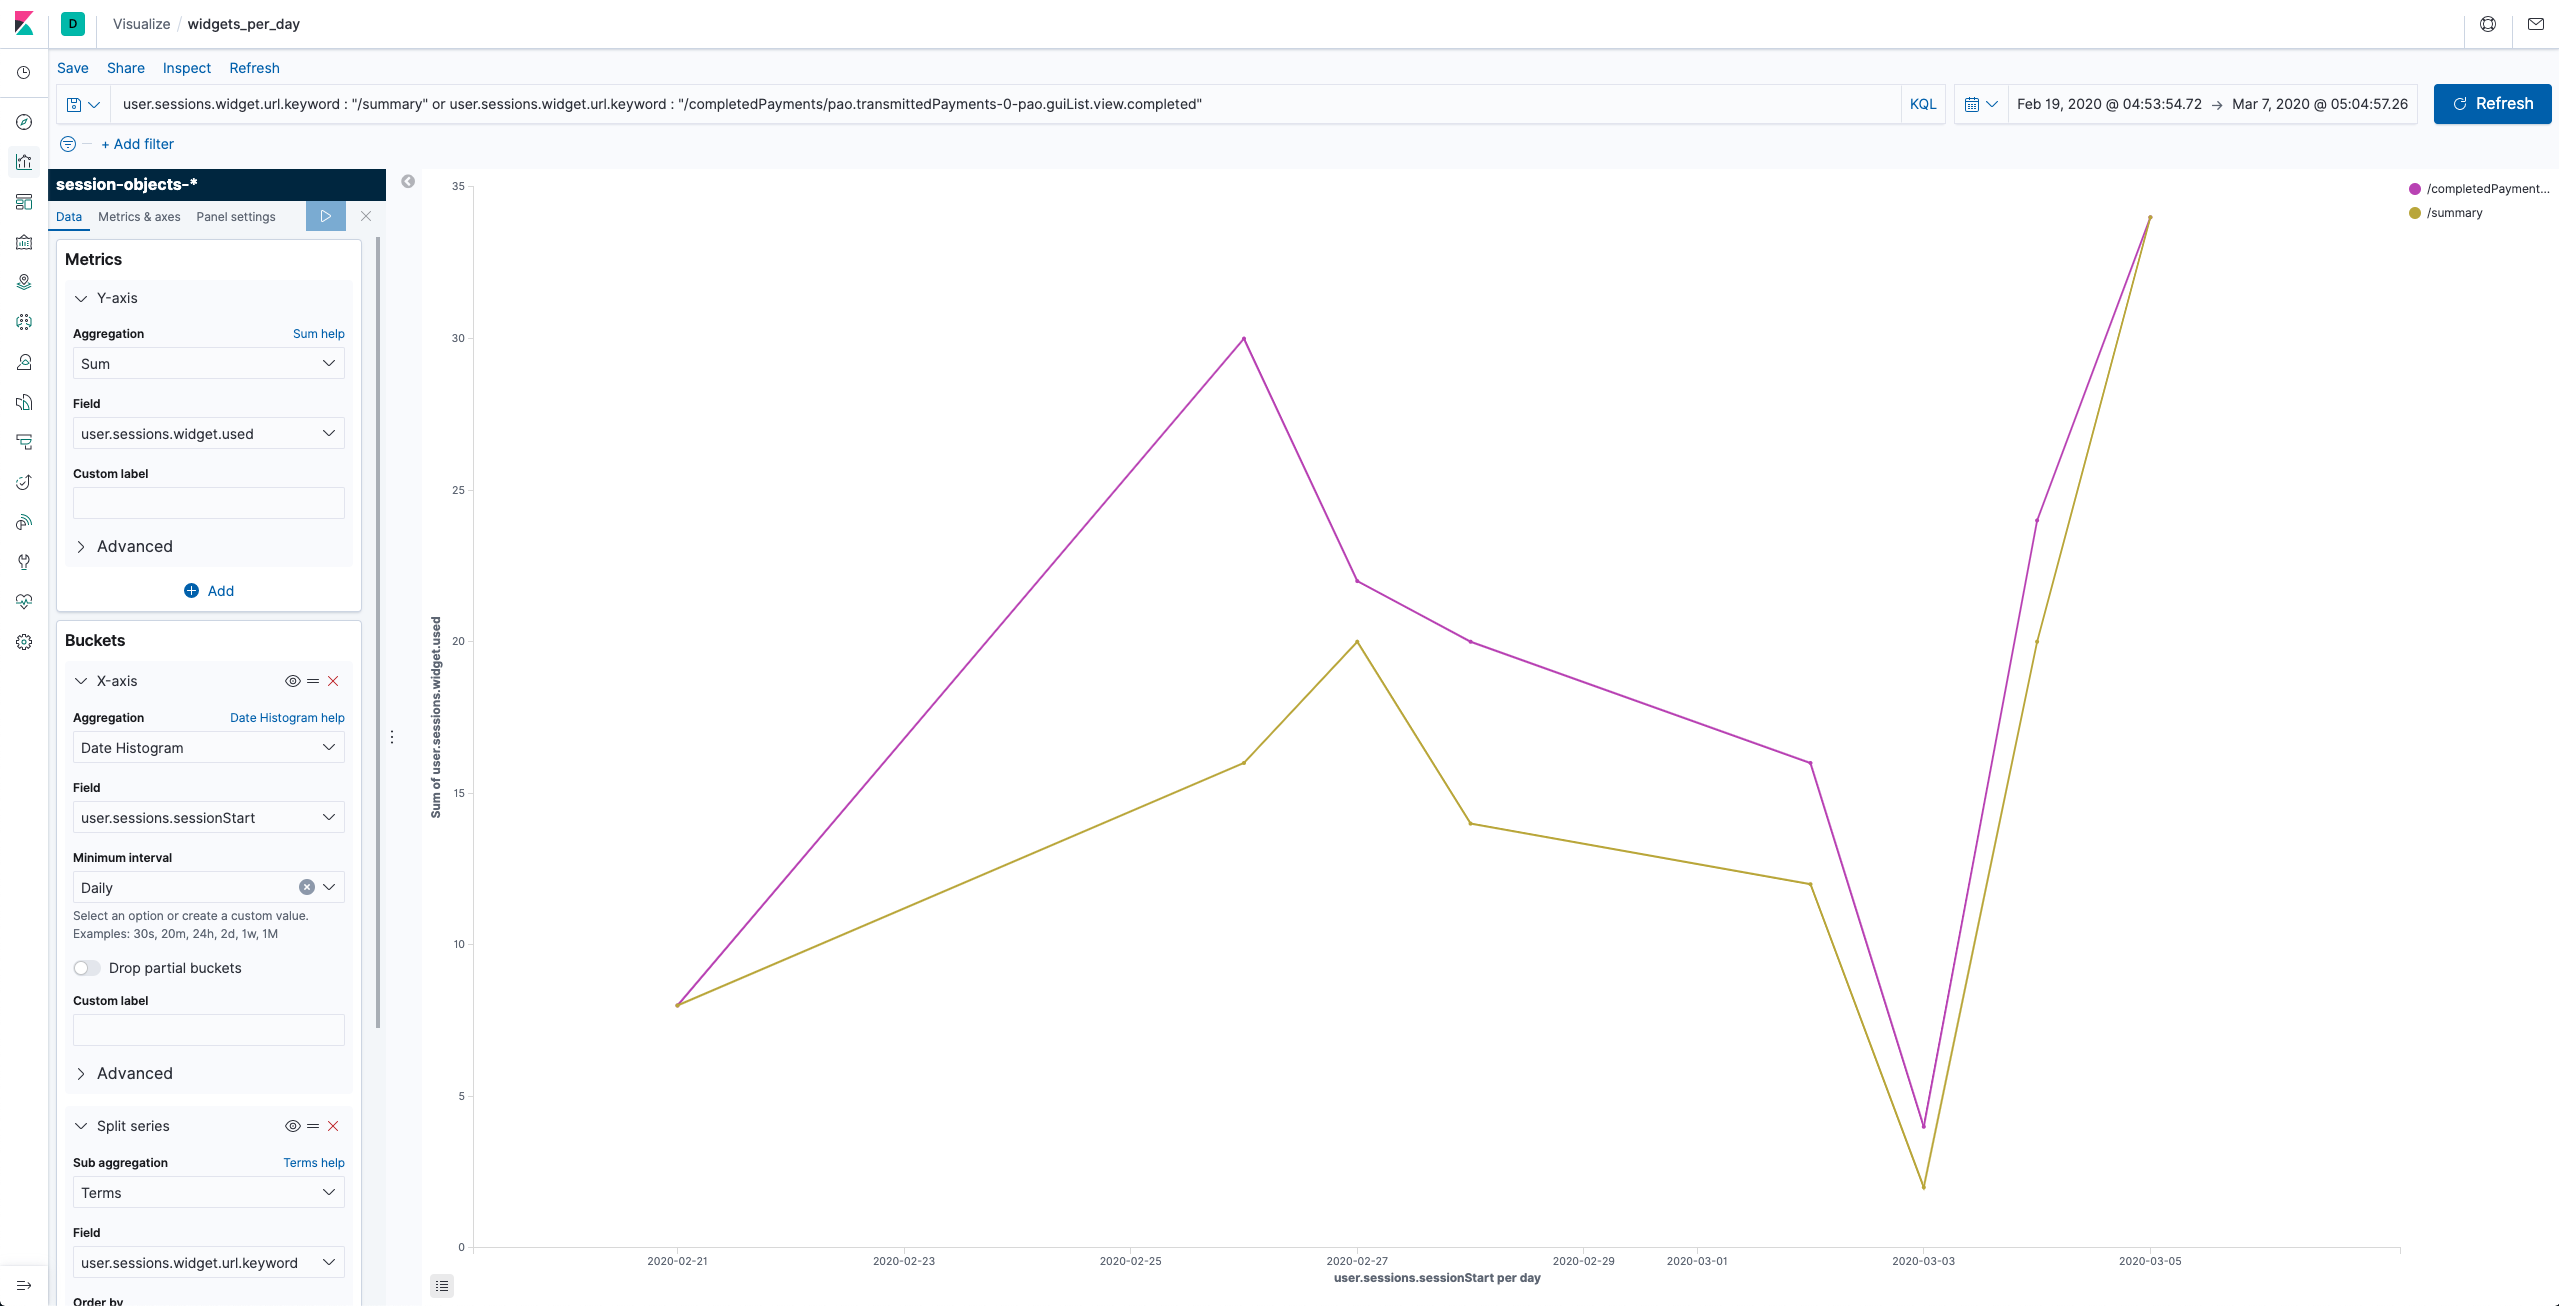
\includegraphics[width=430pt]{bilder/screen_lines.png}
\end{center}
\caption{Lines Visualisierung mit zwei Widgets}
\label{fig:screen_lines}
\end{figure}

\subsubsubsection{Custom Plugin}\\
Um einen erleichterten Einstieg in die Entwicklung eines Custom Plugins zu ermöglichen, bietet Kibana die Möglichkeit, das Grundgerüst für ein Custom Plugin generieren zu lassen \citep{KibPlug20}. Das generierte Plugin liefert direkt die nötige Server-Client-Architektur, um den Elasticsearch-Server anzusprechen. Die grafische Oberfläche, die der Nutzer sieht, ist dabei als Client zu verstehen. Von hier aus werden HTTP Requests an einen Node.js Server gesendet. Dieser kann nun die gesendeten Daten (bspw. eine Suchanfrage) vorbereiten, an den Elasticsearch-Server senden, die Antwort verarbeiten und an den Client weiterleiten. Außerdem ist der Node.js Server auch in der Lage Python Code ausführen zu lassen. Die folgende Abbildung soll diese Beziehung verdeutlichen. 
\begin{figure}[htb]
\begin{center}
	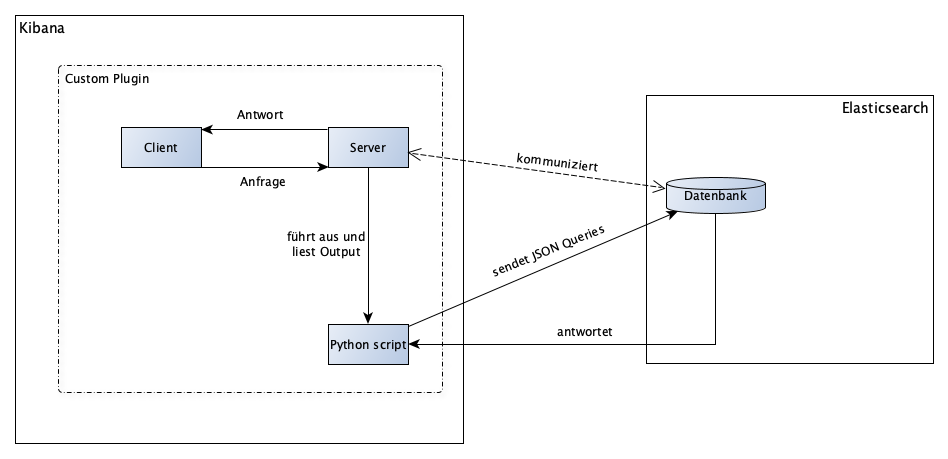
\includegraphics[width=430pt]{bilder/custom_plugin.png}
\end{center}
\caption{Architektur des Custom Plugins}
\label{fig:custom_plugin}
\end{figure}\\
Für den weiteren Verlauf der Arbeit sind die technischen Details der Client-Server-Architektur nicht weiter relevant. Von daher wird nun auf die Implementierung der Python Skripte zur Transformierung der Daten und zur Assoziationsregelanalyse eingegangen.

\subsubsubsection{transform.py}

Das Python Skript zur Transformierung der Daten wird durch das Frontend des Node.js Servers per Button ausgeführt. Bevor die Daten transformiert werden prüft das Skript, ob ein passender Index für die transformierten Daten in Elasticsearch existiert. Ist dies nicht der Fall, wird der entsprechende Index erstellt. Diesem Index wird bei der Erstellung das Mapping vorgegeben, was in Kapitel \ref{ssub:Elasticsearch} erwähnt wurde. Da nun sicher gestellt ist, dass die transformierten Daten korrekt abgespeichert werden, holt sich das Skript eine Liste mit allen verfügbaren Indizes. Aus dieser Liste filtern wir die Indizes, die transformiert werden sollen. An diese Indizes wird nun eine Searchquery gesendet, deren Antwort die transformierten Daten sind. Dabei wollen wir Duplikate und unvollständige Datensätze vermeiden. Ein Duplikat kommt zustande, wenn ein Index zweimal transformiert wird. Da Logstash bzw. Elasticsearch nicht prüft, ob Daten doppelt gespeichert werden, ist es möglich, dieselben Daten mehrmals in einem Index zu speichern. Deshalb prüft das Skript, ob für den Index bereits eine transformierte Datei existiert. Unvollständige Daten können auftreten, indem ein Index zu früh transformiert wird. Es könnte z.B. sein, dass man um 15 Uhr des aktuellen Tages die Daten transformiert, aber später noch neue Daten in den Index gespeichert werden. Würde man den Index zu einem späteren Zeitpunkt nochmal transformieren, hätte man wieder das Problem mit den Duplikaten. Die einfachste Lösung ist demnach, Transformierungen von tagesaktuellen Daten zu unterbinden.\\
Die transformierten Daten werden in demselben Ordner gespeichert, in dem die dazu gehörigen Logfiles liegen. Diese Information ist in dem zu transformierenden Index gespeichert. Dadurch wird sicher gestellt, dass Filebeat die transformierten Daten liest, da auch schon die Logfiles in diesem Ordner gelesen wurden.

\subsubsubsection{associationRuleMiner.py}

In diesem Abschnitt wird die Implementierung des Apriori Algorithmus aus Kapitel \ref{ssub:Klassifizierung} beschrieben. Wie auch in Kapitel \ref{ssub:Klassifizierung} basiert die Implementierung auf den Pseudocode aus \glqq \textit{Knowledge Discovery in Databases}\grqq{} von \citet{EsSa00}.\\
Zu Beginn des Skripts werden der minsupport und die minkonfidenz von der Kommandozeile bzw. von dem Node.js Server, der das Skript ausführt, eingelesen. Um eine Verbindung zu Elasticsearch aufzubauen, wird das Modul \textproc{elasticsearch} benutzt. Als Nächstes wird über den Elasticsearch-Client die Größe der Datenbank\footnote{Datenbank wird in diesem Fall als Synonym für Anzahl an Sessions benutzt.} und eine Liste an benutzten Widgets ermittelt. Die Liste der Widgets wird als \textproc{Set} gespeichert und die Elemente als \textproc{frozenset}. Das hat den Vorteil, dass wir nun eine Kandidatenmenge haben, die aus einelementigen Mengen besteht. Aus dieser Menge werden nun mit dem Apriori Algorithmus die häufigen Itemsets ermittelt.\\
Erwähnenswert ist an dieser Stelle die Funktion \textit{joinSets}. Anhand des folgenden Codeausschnitts wird die Funktionsweise erläutert.
\clearpage
\begin{figure}[htb]
\lstinputlisting[language=Python, xleftmargin=2.5em,frame=single,framexleftmargin=2.2em,firstline=85, lastline=114,basicstyle=\scriptsize, caption=joinSets aus associationRuleMiner.py,captionpos=b,label=lst:code-snippet-joinsets]{../python/associationRuleMiner.py}
\end{figure}
In Zeile 15 - 28 wird mit Hilfe eines Iterators durch die Menge iteriert, deren Elemente die Länge $k$ haben. Das erste Element der Menge wird dabei in der Variable \textit{startItem} gespeichert. Nun wird für jedes weitere Element der Menge geprüft, ob die beiden Mengen miteinander vereinigt werden können. Die Voraussetzung dafür ist, dass beide Mengen $k-1$ gleiche Elemente haben. Diese Voraussetzung wird in Zeile 22 geprüft. Wenn der Durchschnitt der beiden Mengen die Länge $k-1$ hat, bedeutet das, dass die beiden Mengen genau $k-1$ Elemente haben. Also dürfen diese Mengen vereinigt und in \textit{newCandidatesSet} gespeichert werden. Wenn alle Elemente durchlaufen wurden, wird das \textit{startElement} aus der Menge über die iteriert wird gelöscht. Dadurch steht das ursprünglich zweite Element an erster Stelle. Der Iterator wird entsprechend aktualisiert und es wird versucht, dieses Element mit einem anderen zu vereinigen. Hier wird nun deutlich, worin der Vorteil bei der Wahl von \textproc{set} und \textproc{frozenset} als Datentyp liegt: durch die Mengenoperationen wurde vermieden, dass die Mengen elementweise verglichen werden müssen.\footnote{Python implementiert \textproc{set}s als Hash Tables. Intern werden z.B. bei der Vereinigung von Mengen auch Elemente miteinander verglichen \citep{GeFoGe20}. Aber da es sich um Hash Tables handelt, geht dies schneller, als würde man das selber implementieren. Außerdem ist durch die Hash Tables gegeben, dass Elemente effizient gesucht werden können.}\\
Anschließend muss für die vereinigten Mengen geprüft werden, ob alle ihrer Teilmengen häufig sind. Dazu berechnet die Funktion \textproc{it.combinations} aus dem Modul \textproc{itertools} alle $k-1$ elementigen Teilmengen. Für jede Teilmenge wird geprüft, ob sie in der Menge der häufigen Itemsets enthalten ist. Ist dies nicht der Fall wird das Element, das die Teilmenge beinhaltet gelöscht. Daraus resultiert die neue Kandidatenmenge, für die der Support geprüft wird.\\
Nachdem die häufigen Itemsets bestimmt wurden, werden alle Regeln gesucht, die die minkonfidenz erfüllen. Die Implementierung dazu zeigt Listing \ref{lst:code-snippet-generateRules}.\\
\begin{figure}[htb]
%\lstinputlisting[language=Python, firstline=165, lastline=192,basicstyle=\scriptsize, caption=generateRules aus associationRuleMiner.py,captionpos=b,label=lst:code-snippet-generateRules]{../python/associationRuleMiner.py}
	\begin{lstlisting}[language=python,xleftmargin=2.5em,frame=single,framexleftmargin=2.2em, basicstyle=\scriptsize, caption=generateRules aus associationRuleMiner.py,captionpos=b,label=lst:code-snippet-generateRules]
def generateRules(freqItems, antecedenceItems, resultSet):
    """ This function generates all possible association rules that can be found in the frequent itemsets that satisfy
        the minconf. Like the minsupport the minconf need to be passed by the command line using -minconf=[value].
        The confidence of a rule A => X - A is calculated as support(X) / support(A). If this rule satisfies the
        minconf it will check if A' also satisfies the minconf where A' is a subset of A. This is done recursively
        at the end of the function.

    Args:
        freqItems (set): Set of frequent items in which association rules should be found
        antecedenceItems (set): Set of items that are a a subset of the itemset of the left side of an association rule
        resultSet (set): Set of found association rules

    """
    for item in antecedenceItems:
        item = antecedenceItems.difference(frozenset([item]))

        supportItemset = getCount(freqItems) / dbsize
        supportItem = getCount(item) / dbsize

        confidence = supportItemset / supportItem

        if confidence >= float(args.minconf):
            consequence = freqItems.difference(item)
            resultStr = f'{list(item)}->{list(consequence)},' \
                         f'support:{format(supportItemset,".4f")},confidence:{format(confidence,".4f")}'
            resultSet.add(resultStr)
            if len(item) > 1:
                generateRules(freqItems, item, resultSet)

for frequentItem in frequentItems:
	generateRules(frequentItem, frequentItem, resultSet)
	\end{lstlisting}
\end{figure}\\
Initial wird die Funktion \textproc{generateRules} mit einem häufigen Itemset aufgerufen, wobei dieses Itemset zweimal als Argument übergeben wird. Da wir Regeln der Form 
\begin{equation*}
	Y \rightarrow X - Y, Y \subseteq X
\end{equation*}
bilden wollen, wird die Menge $Y$ (Zeile 1: \textit{antecedenceItems}) elementweise durchlaufen und die Differenz zur Menge $X$ (Zeile 1: \textit{freqItems}) gebildet (Zeile 15). Die Konfidenz solch einer Regel kann nach \citet{EsSa00} durch 
\begin{equation*}
	\text{konfidenz(}Y \rightarrow (X-Y)\text{)} = \frac{\text{support(X)}}{\text{support(Y)}}
\end{equation*}
berechnet werden (Zeile 20). Falls diese Regel die Konfidenz erfüllt, wird dies in \mbox{\textproc{resultItem}} gespeichert. Anschließend werden rekursiv Regeln für $Y'$, $Y' \subset Y$ gesucht.
%\textbf{Custom Plugin}\\\\
%Kibana bietet aber nicht ohne Weiteres die Möglichkeit, einen Workflow zu erkennen, wie es in der zweiten Frage aus Kapitel \ref{sub:Problemstellung} gefordert ist. Deshalb wurde im Zuge der Arbeit ein Custom Plugin für Kibana entworfen.


\clearpage
